% Recommended preamble:
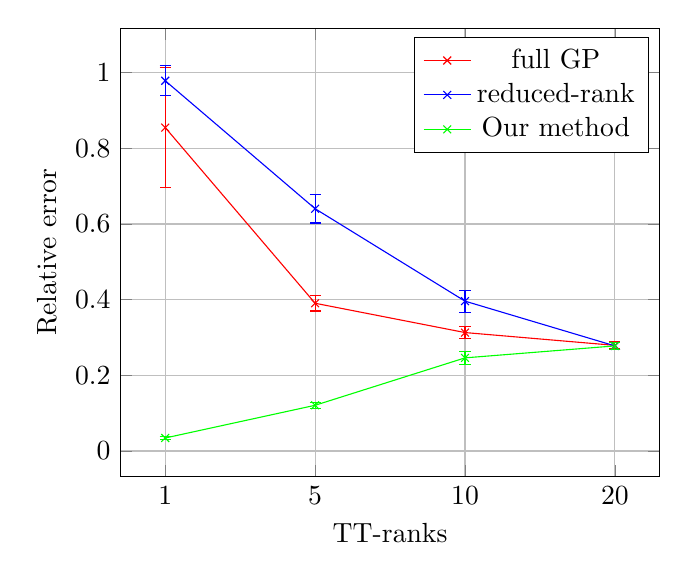
\begin{tikzpicture}
\begin{axis}[xmajorgrids, ymajorgrids, xlabel={TT-ranks}, ylabel={Relative error}, xtick={1,2,3,4}, xticklabels={1,5,10,20}]
    \addplot[color={red}, mark={x}, error bars/y dir=both, error bars/y explicit]
        coordinates {
            (1,0.8548488000000003) +- (0,0.15855295627560317)
            (2,0.3905046) +- (0,0.02058131212856297)
            (3,0.31306750000000005) +- (0,0.015708690427417696)
            (4,0.27919499999999997) +- (0,0.009568455895400384)
        }
        ;
    \addplot[color={blue}, mark={x}, error bars/y dir=both, error bars/y explicit]
        coordinates {
            (1,0.9786296) +- (0,0.04006252166080191)
            (2,0.6403738000000001) +- (0,0.037763301211626056)
            (3,0.39609749999999994) +- (0,0.029091398615207355)
            (4,0.27780689999999997) +- (0,0.009028143853159042)
        }
        ;
    \addplot[color={green}, mark={x}, error bars/y dir=both, error bars/y explicit]
        coordinates {
            (1,0.03444092000000001) +- (0,0.0031263041370495825)
            (2,0.120855) +- (0,0.0075953653851104095)
            (3,0.2461954) +- (0,0.016573944941785386)
            (4,0.27780689999999997) +- (0,0.009028143853159042)
        }
        ;
    \legend{{full GP},{reduced-rank},{Our method}}
\end{axis}
\end{tikzpicture}
